\documentclass[14pt]{extreport}
\usepackage{cmap}
\usepackage[utf8]{inputenc}
\usepackage[english,ukrainian]{babel}
\usepackage{graphicx}
\usepackage{geometry}
\usepackage{listings}
\usepackage{amsmath}
\usepackage{float}
\geometry{
	a4paper,
	left=20mm,
	right=20mm,
	top=20mm,
	bottom=20mm
}
\lstset{
	language=bash,
	tabsize=4,
	breaklines,
	keepspaces,
	showstringspaces=false,
}
\graphicspath{ {./pictures} }
\setlength{\parindent}{4em}

\newcommand\subject{Кросплатформне програмування}
\newcommand\lecturer{доцент кафедри ПЗ\\Дяконюк Л.М.}
\newcommand\teacher{ст. викл. кафедри ПЗ\\Шкраб Р.Р.}
\newcommand\mygroup{ПЗ-32}
\newcommand\lab{2}
\newcommand\theme{Робота з класами. Наслідування,
	поліморфізм. Створення класу-обгортки для
	колекції екземплярів. Сортування та пошук
}
\newcommand\purpose{Навчитися працювати з класами. Наслідування,
	поліморфізм. Створення класу-обгортки для
	колекції екземплярів. Сортування та пошук}

\begin{document}
\begin{normalsize}
	\begin{titlepage}
		\thispagestyle{empty}
		\begin{center}
			\textbf{МІНІСТЕРСТВО ОСВІТИ І НАУКИ УКРАЇНИ\\
				НАЦІОНАЛЬНИЙ УНІВЕРСИТЕТ "ЛЬВІВСЬКА ПОЛІТЕХНІКА"}
		\end{center}
		\begin{flushright}
			Інститут \textbf{КНІТ}\\
			Кафедра \textbf{ПЗ}
		\end{flushright}
		\vspace{160pt}
		\begin{center}
			\textbf{ЗВІТ}\\
			\vspace{10pt}
			До лабораторної роботи № \lab\\
			\textbf{На тему}: “\textit{\theme}”\\
			\textbf{З дисципліни}: “\subject”
		\end{center}
		\vspace{40pt}
		\begin{flushright}
			
			\textbf{Лектор}:\\
			\lecturer\\
			\vspace{10pt}
			\textbf{Виконав}:\\
			
			студент групи \mygroup\\
			Коваленко Д.М.\\
			\vspace{10pt}
			\textbf{Прийняв}:\\
			
			\teacher\\
			
			\vspace{28pt}
			«\rule{1cm}{0.15mm}» \rule{1.5cm}{0.15mm} 2023 р.\\
			$\sum$ = \rule{1cm}{0.15mm}……………\\
			
		\end{flushright}
		\vspace{\fill}
		\begin{center}
			\textbf{Львів — 2023}
		\end{center}
	\end{titlepage}
		
	\begin{description}
		\item[Тема.] \theme.
		\item[Мета.] \purpose.
	\end{description}
	

	\section*{Лабораторне завдання}
	Житло Визначити ієрархію житла, наприклад: особняк, квартира, пентхаус і т.д.
	Сформувати пропозиції наявного житла в м. Львові для покупця. Врахувати
	розташування житла до об’єктів соціальної інфраструктури (садочки, школи, дитячі
	майданчики)
	Реалізувати можливість сортування знайдених опцій житла за двома типами
	параметрів (на вибір, реалізовано як два окремі методи)
	Реалізація сортування має передбачати можливість сортувати як за спаданням, так
	і за зростанням
	
	\section*{Хід роботи}

	\textbf{\textit{Main.java}}
	\begin{lstlisting}
import java.util.ArrayList;
import java.util.Comparator;
import java.util.List;
abstract class Housing {
	private String name;
	private int distanceToSchool;
	private int distanceToPark;
	
	public Housing(String name, int distanceToSchool, int distanceToPark) {
		this.name = name;
		this.distanceToSchool = distanceToSchool;
		this.distanceToPark = distanceToPark;
	}
	
	public String getName() {
		return name;
	}
	
	public int getDistanceToSchool() {
		return distanceToSchool;
	}
	
	public int getDistanceToPark() {
		return distanceToPark;
	}
	
	@Override
	public String toString() {
		return "Housing{" +
			"name='" + name + '\'' +
			", distanceToSchool=" + distanceToSchool +
			", distanceToPark=" + distanceToPark +
			'}';
	}
}
class Townhouse extends Housing {
	private int numberOfFloors;
	
	public Townhouse(String name, int distanceToSchool, int distanceToPark, int numberOfFloors) {
		super(name, distanceToSchool, distanceToPark);
		this.numberOfFloors = numberOfFloors;
	}
	
	public int getNumberOfFloors() {
		return numberOfFloors;
	}
	
	@Override
	public String toString() {
		return super.toString() + "\nNumber of Floors: " + numberOfFloors;
	}
}

// Subclass for Mansion
class Mansion extends Housing {
	private int numberOfBathrooms;
	
	public Mansion(String name, int distanceToSchool, int distanceToPark, int numberOfBathrooms) {
		super(name, distanceToSchool, distanceToPark);
		this.numberOfBathrooms = numberOfBathrooms;
	}
	
	public int getNumberOfBathrooms() {
		return numberOfBathrooms;
	}
	
	@Override
	public String toString() {
		return super.toString() + "\nNumber of Bathrooms: " + numberOfBathrooms;
	}
}

class Condo extends Housing {
	private int floorNumber;
	private boolean hasAmenities;
	
	public Condo(String name, int distanceToSchool, int distanceToPark, int floorNumber, boolean hasAmenities) {
		super(name, distanceToSchool, distanceToPark);
		this.floorNumber = floorNumber;
		this.hasAmenities = hasAmenities;
	}
	
	public int getFloorNumber() {
		return floorNumber;
	}
	
	public boolean hasAmenities() {
		return hasAmenities;
	}
	
	@Override
	public String toString() {
		return super.toString() + "\nFloor Number: " + floorNumber + "\nHas Amenities: " + (hasAmenities ? "Yes" : "No");
	}
}


class HousingManager {
	List<Housing> housings;
	
	HousingManager(List<Housing> housings) {
		this.housings = housings;
	}
	
	static class sortByDistanceToSchoolAsc implements Comparator<Housing> {
		@Override
		public int compare(Housing h1, Housing h2) {
			return Integer.compare(h1.getDistanceToSchool(), h2.getDistanceToSchool());
		}
	}
	
	class sortByDistanceToParkAsc implements Comparator<Housing> {
		@Override
		public int compare(Housing h1, Housing h2) {
			return Integer.compare(h1.getDistanceToPark(), h2.getDistanceToPark());
		}
	}
	
	public static Comparator<Housing> sortByDistanceToSchoolDesc() {
		return new Comparator<Housing>() {
			@Override
			public int compare(Housing h2, Housing h1) {
				return Integer.compare(h1.getDistanceToSchool(), h2.getDistanceToSchool());
			}
		};
	}
	
	public static Comparator<Housing> sortByDistanceToParkDesc() {
		return (h2, h1) -> Integer.compare(h1.getDistanceToPark(), h2.getDistanceToPark());
	}
}

public class Main {
	public static void main(String[] args) {
		List<Housing> housingList = new ArrayList<>();
		housingList.add(new Condo("Condo A", 2, 1, 5, true));
		housingList.add(new Mansion("Mansion B", 1, 5, 1));
		housingList.add(new Townhouse("Townhouse C", 4, 3, 2));
		HousingManager mgr = new HousingManager(housingList);
		
		// Sort by distance to school (ascending) using static inner class
		housingList.sort(new HousingManager.sortByDistanceToSchoolAsc());
		System.out.println("Sorted by distance to school (ascending):");
		System.out.println(housingList);
		
		// Sort by distance to park (ascending) using inner class
		housingList.sort(mgr.new sortByDistanceToParkAsc());
		System.out.println("\nSorted by distance to park (ascending):");
		System.out.println(housingList);
		
		// Sort by distance to school (descending) using anonymous inner class
		housingList.sort(HousingManager.sortByDistanceToSchoolDesc());
		System.out.println("\nSorted by distance to school (descending):");
		System.out.println(housingList);
		
		// Sort by distance to park (descending) using lambda expressions
		housingList.sort(HousingManager.sortByDistanceToParkDesc());
		System.out.println("\nSorted by distance to park (descending):");
		System.out.println(housingList);
	}
}

	\end{lstlisting}	
	
	
	\begin{figure}[H]
		\centering
		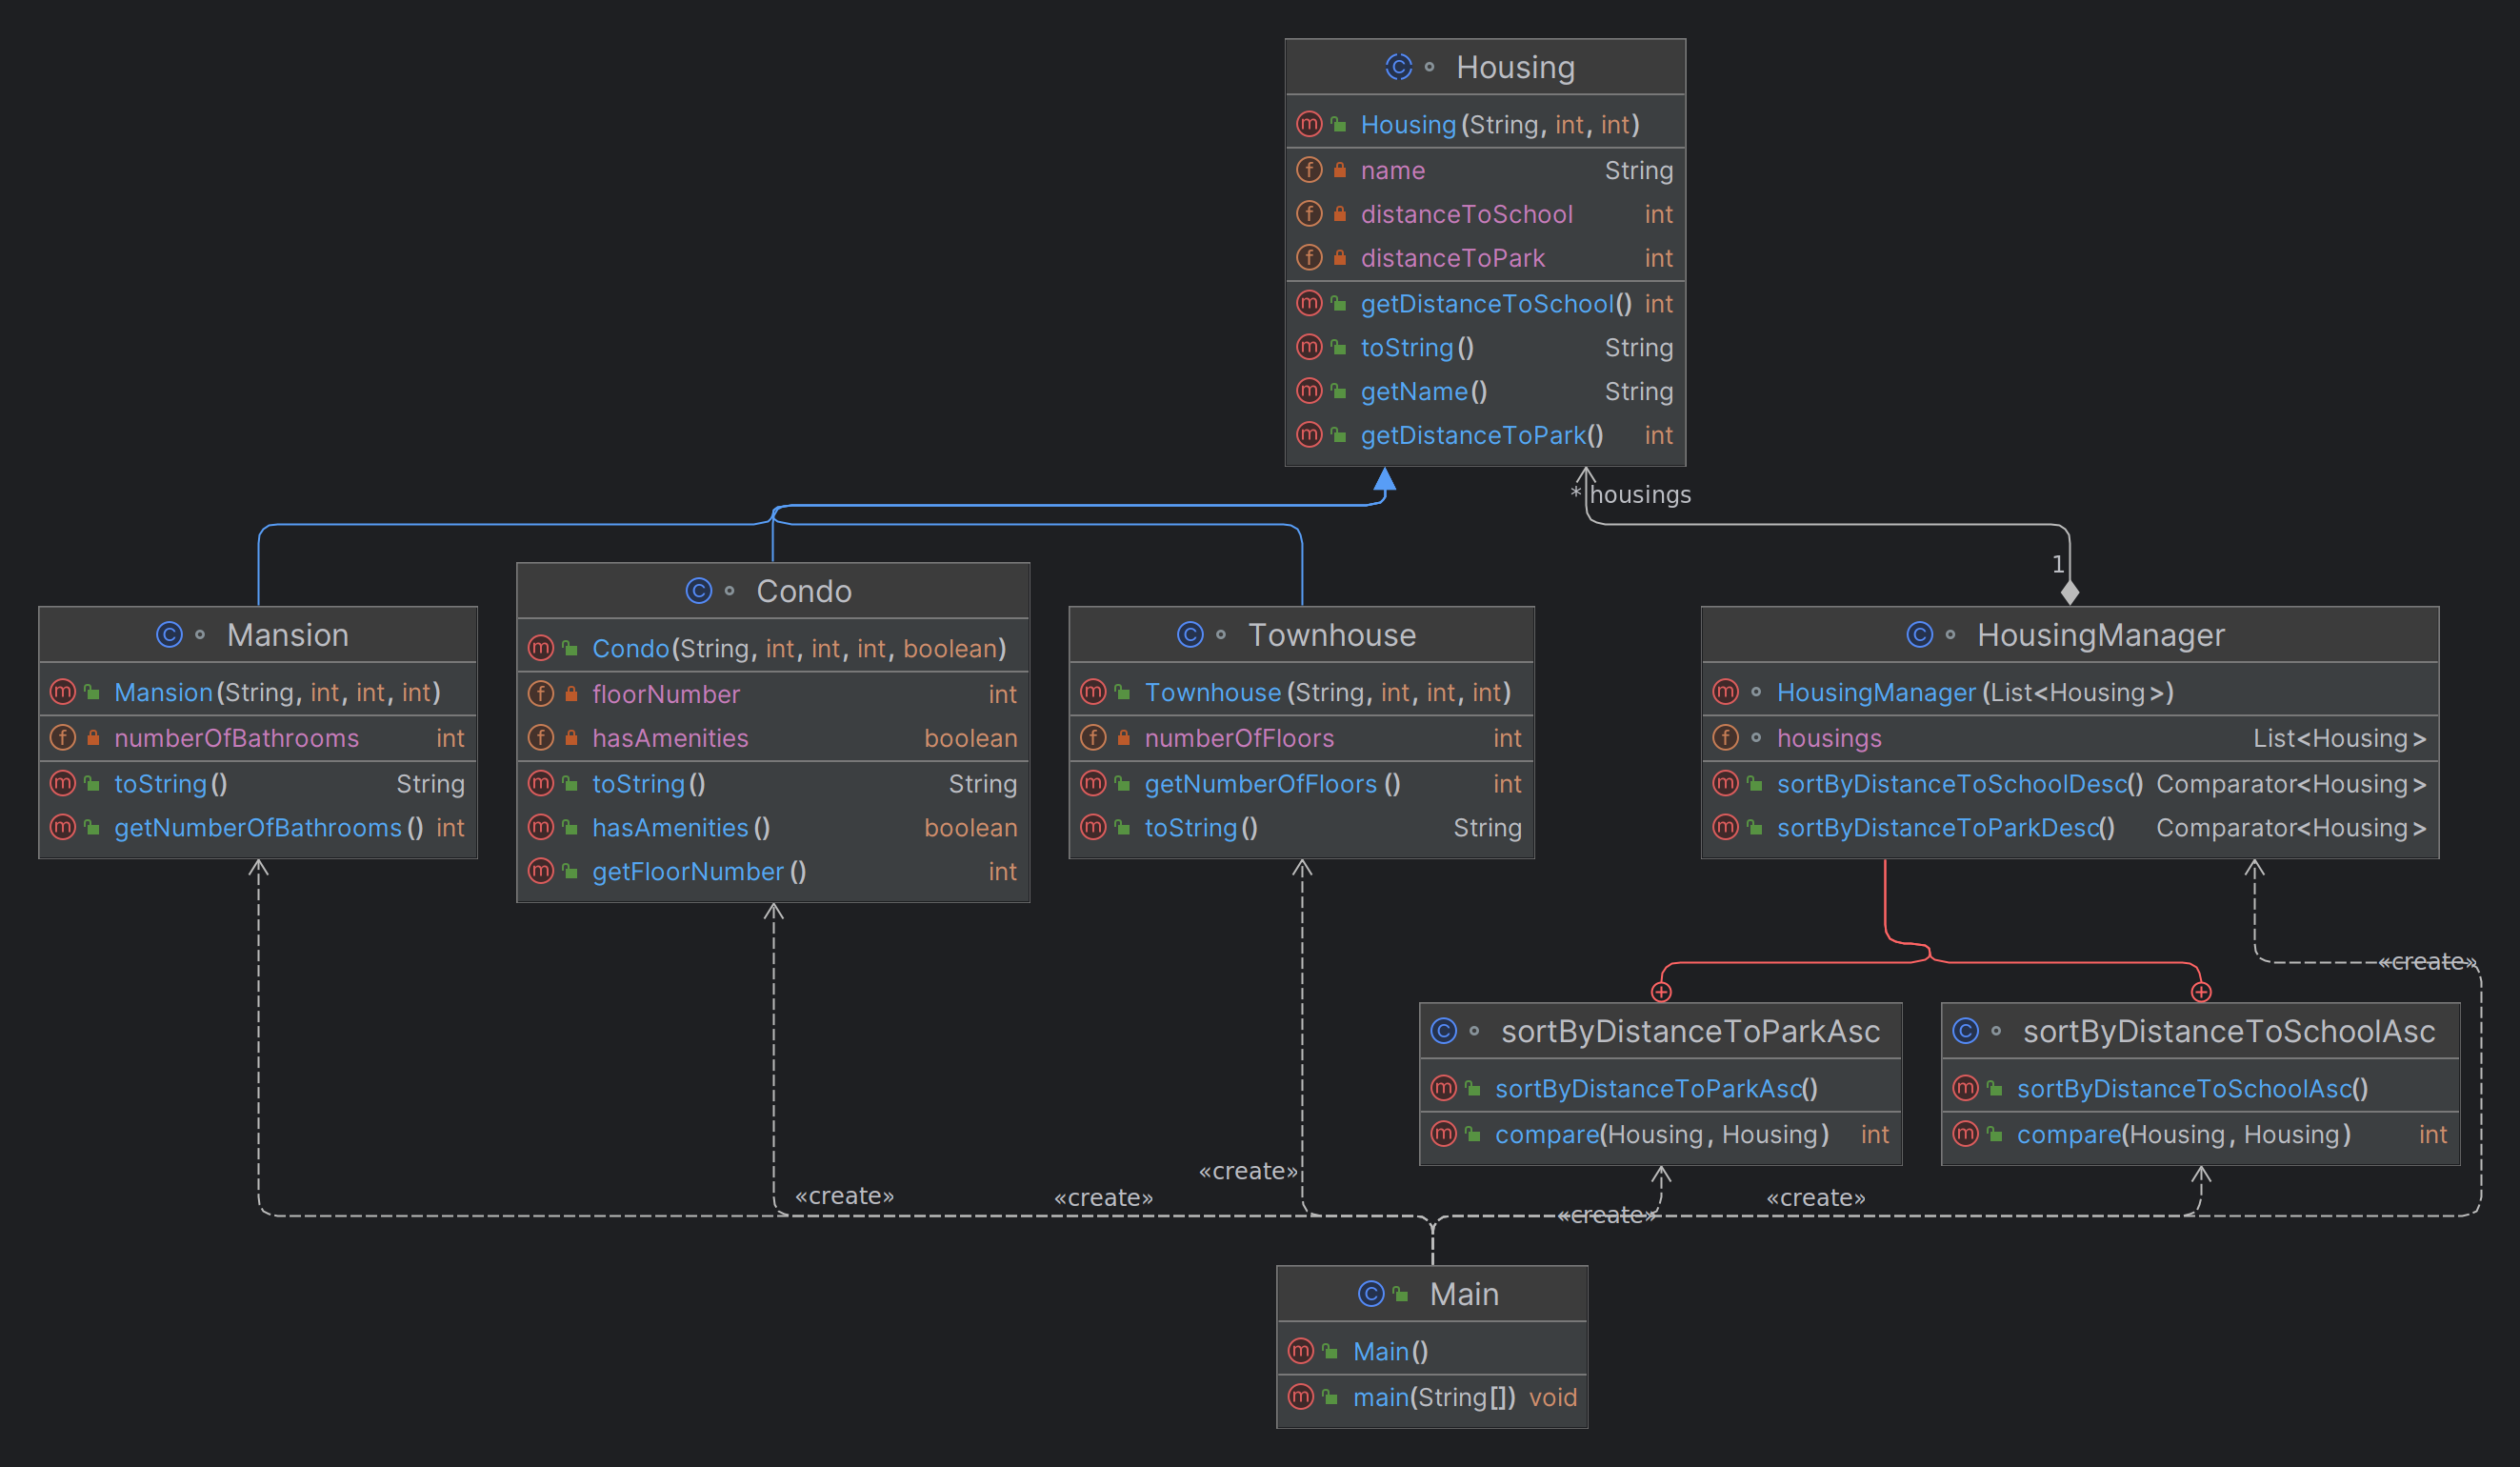
\includegraphics[scale=0.18]{2}
		\caption{Діаграма класів}
	\end{figure}
	
	\begin{figure}[H]
		\centering
		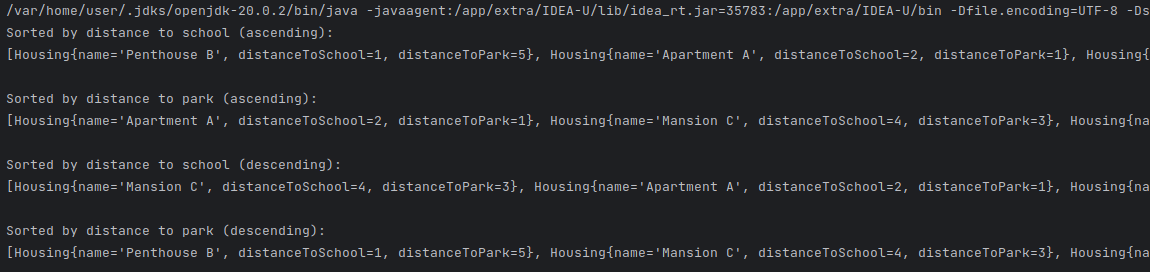
\includegraphics[scale=0.4]{1}
		\caption{Робота програми}
	\end{figure}

	\section*{Висновок}
	Під час виконання лабораторної роботи я працював з класами. Реалізував наслідування, поліморфізм. Створив клас-обгортки для
	колекції екземплярів.
	 
\end{normalsize}
\end{document}
